\chapter{Statistics}

\section{Q1}

  \begin{figure}[H]
    \centering
    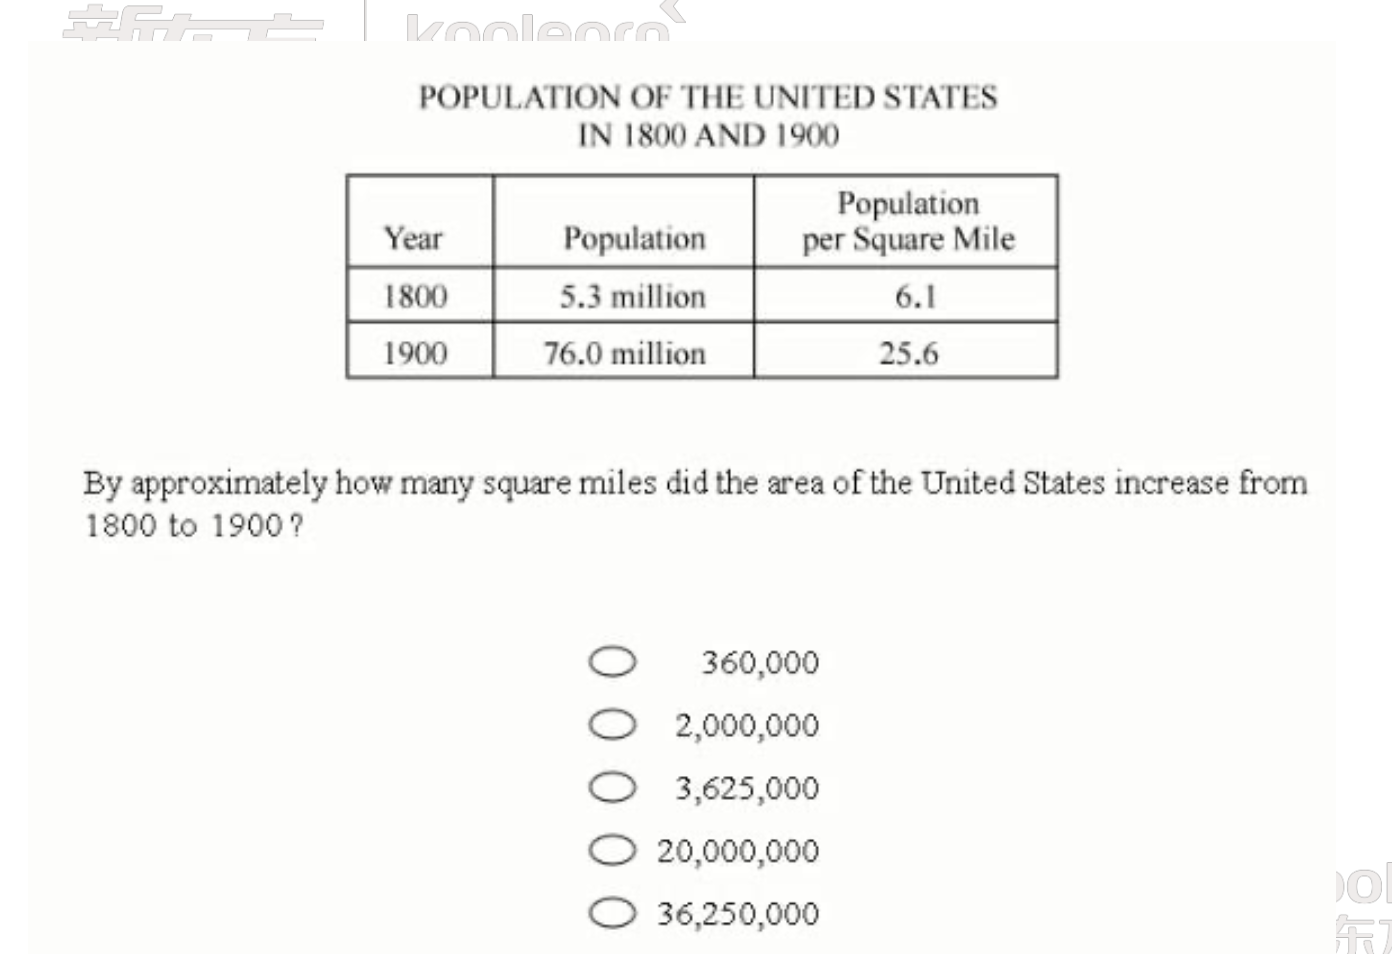
\includegraphics[width=0.7\columnwidth]{images/areas/stats/q1.png}
  \end{figure}

  \subsection{解析}

    \begin{equation*}
      A = \frac{\text{population}}{\text{population per square miles}}
    \end{equation*}

    \textbf{B}

\section{Q2}

  \begin{figure}[H]
    \centering
    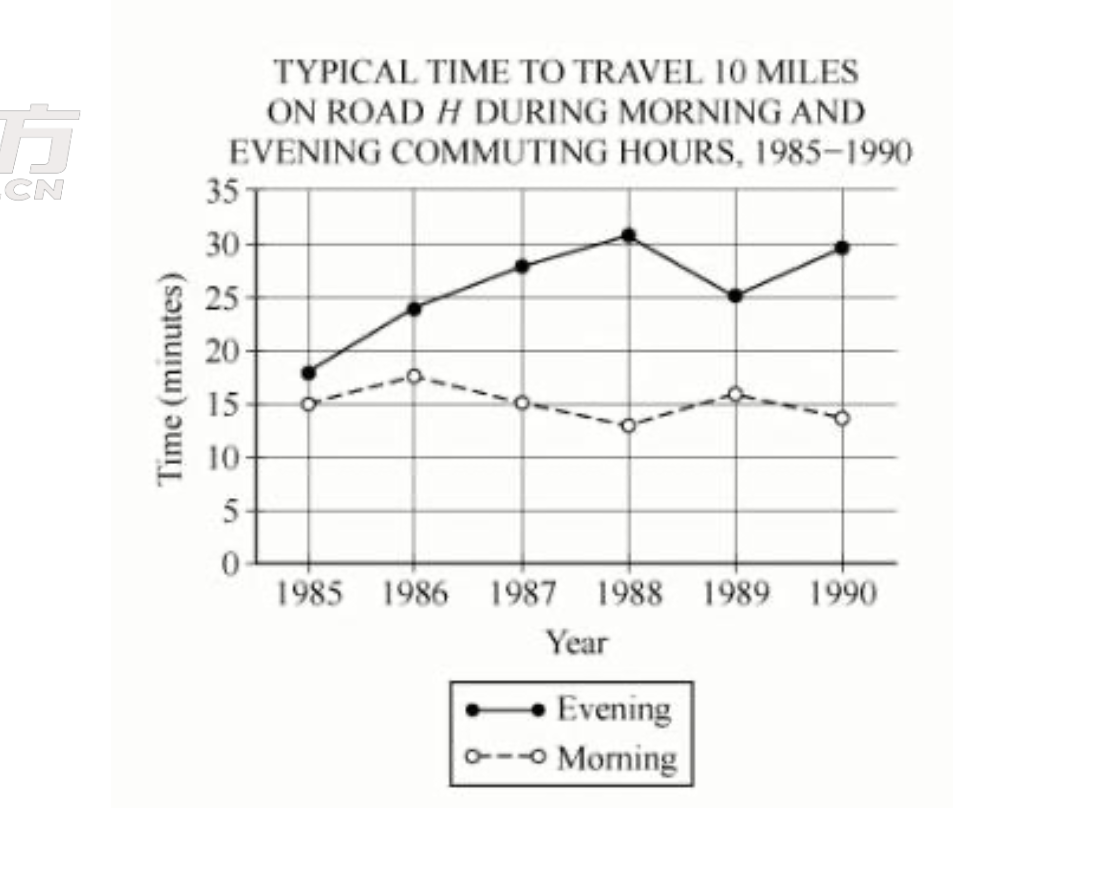
\includegraphics[width=0.7\columnwidth]{images/areas/stats/q2.png}
  \end{figure}

  The typical travel time during the morning commuting hours decreased by
  approximately what percent from 1986 to 1998?

  \begin{enumerate}
    \item 5\%
    \item 10\%
    \item 25\%
    \item 40\%
    \item 45\%
  \end{enumerate}

  \subsection{解析}

    \textbf{C}: 这种题要通过约分来做, 约分后1986年是20, 1988年是15. 所以下降百分之25

\section{Q3}

  Martha invited 4 friends to go with her to the movies. There are 120
  different ways in which they can sit together in a row of 5 seats,
  one person per seat. In how many of those ways is Martha sitting in the
  middle seat?

  \subsection{解析}

    Martha坐中间, 所以先让Martha做

    \begin{equation*}
      4 \times 3 \times 2 \times 1 = 24
    \end{equation*}

\section{Q4}

  From a box of 10 light bulbs, you are to remove 4. How many different sets
  of 4 light bulbs could you remove?

  \subsection{解析}

    \begin{align*}
      n &= 10 \\
      r &= 4 \\
      s &= \frac{10!}{4!\left( 10 - 4 \right)!} \\
      &= 210
    \end{align*}

\section{Q5}

  In a box of 10 electrical parts, 2 are defective.

  \begin{enumerate}
    \item If you choose one part at random from the box, what is the
    probability that it is not defective?
    \item If you choose two parts at random from the box, without replacement,
    what is the probability that both are defective?
  \end{enumerate}

  \subsection{解析}

    \begin{enumerate}
      \item $ \frac{4}{5} $
      \item $ \frac{1}{45} $
    \end{enumerate}

\section{Q6}

  Lin and Mark each attempt independently to decode a message.
  If the probability that Lin will decode the message is 0.80 and the
  probability that Mark will decode the message is 0.70,
  find the probability that

  \begin{enumerate}
    \item at least one of them will decode the message
  \end{enumerate}

  \subsection{解析}

    都没找到的可能性是

    \begin{equation*}
      \left( 1 - 0.8 \right) \times \left( 1 - 0.7 \right) = 0.06
    \end{equation*}

    只要一个人找到是都没找到的反面, 所以

    \begin{equation*}
      1 - 0.06 = 0.94
    \end{equation*}

\section{Q7}

  \begin{figure}[H]
    \centering
    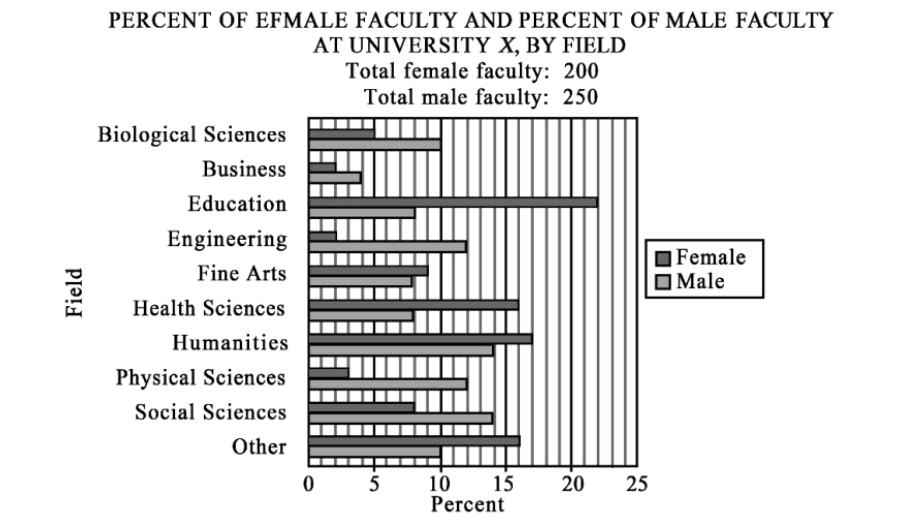
\includegraphics[width=0.7\columnwidth]{images/areas/stats/q7.png}
  \end{figure}

  Approximately what percent of the faculty in humanities are male?

  \subsection{解析}

    \textbf{本题男女总人数不一样, 所以要先算humanities的男女人数}

    \begin{align*}
      \frac{0.14 * 250}{0.17 * 200 + 0.14 * 250}
      &= \frac{35}{34 + 35} \\
      &\approx 0.51
    \end{align*}

\section{Q8}

  The sum of n numbers is greater than 48. If the average (arithmetic mean)
  of n numbers is 1.2, what is the least possible value of n?

  \subsection{解析}

    \textbf{本题注意审题, \say{greater than}}

    \begin{align*}
      \text{mean } &= \frac{\text{sum}}{n} \\
      1.2 &= \frac{48}{n} \\
      n &= 40
    \end{align*}

    应为\say{is greater than 48}, 所以选 $ 41 $

\section{Q9}

  If the average (arithmetic mean) of x, y, z, 5 and 7 is 8, which of the
  following must be true?

  \begin{enumerate}
    \item The median of the five numbers cannot be 5.
    \item At least one of x, y and z is greater than 9.
    \item The range of the five numbers is 2 or more.
  \end{enumerate}

  \subsection{解析}

    \begin{itemize}
      \item \textbf{错误}: 如果 $ x, y = 0 $, $ z $ 为一个极大的数, median就可以是5
      \item \textbf{正确}: xyz没有限制
      \item \textbf{正确}: 5, 7的range已经是2
    \end{itemize}

\section{Q10}

  The range of the heights of the female students in a certain class is 13.2
  inches, and the range of the heights of the male students in the class is
  15.4 inches. Which of the following statements individually provide(s)
  sufficient additional information to determine the range of the heights
  of all the students in the class? Indicate all such statements.

  \begin{enumerate}
    \item The tallest male student in the class is 5.8 inches taller than the
    tallest female student in the class.
    \item B. The median height of the male students in the class is 1.1 inches
    greater than the median height of the female students in the class.
    \item C. The average (arithmetic mean) height of the male students in the
    class is 4.6 inches greater than the average height of the female students
    in the class.
  \end{enumerate}

  \subsection{解析}

    \begin{enumerate}
      \item \textbf{正确}:
      \begin{align*}
        M_{t} &= M \\
        F_{t} &= M - 5.8 \\
        M_{s} &= M - 15.4 \\
        F_{s} &= M - 5.8 - 13.2 \\
        &= M - 19.0 \\
        R &= M - \left( M - 19.0 \right)
      \end{align*}
      \item \textbf{错误}: 不知道总数
      \item \textbf{错误}: 不知道总数
    \end{enumerate}

\section{Q11}

  The company at which Mark is employed has 80 employees, each of whom has a
  different salary. Mark’s salary of 43,700 is the second-highest salary
  in the first quartile of the 80 salaries. If the company were to hire
  8 new employees at salaries that are less than the lowest of the 80 salaries,
  what would Mark’s salary be with respect to the quartiles of the 88 salaries
  at the company, assuming no other changes in the salaries?

  \subsection{解析}

    \say{first quartile}的second lowest说明排名倒数19. 末尾加8人排名27, 得到
    \say{The fifth-lowest salary in the second quartile}

    \textbf{first quartile}是最低的半分之25

\section{Q12}

  Each of the following linear equations defines y as a function of x for all
  integers x from 1 to 100. For which of the following equations is the
  standard deviation of the y-values corresponding to all the x-values the
  greatest?

  \begin{enumerate}
    \item $ y = \frac{x}{3} $
    \item $ y = \frac{x}{2} + 10 $
    \item $ y = x $
    \item $ y = 2x + 50 $
    \item $ y = 3x - 20 $
  \end{enumerate}

  \subsection{解析}

    Standard deviation测量数据和平均数的差距, $ y = 3x - 20 $的跨度最大

\section{Q13}

  A random variable Y is normally distributed with a mean of 200 and a standard
  deviation of 10.

  \begin{itemize}
    \item \textbf{Quantity A}: The probability of the event that the value of Y
    is greater than 220
    \item \textbf{Quantity B}: $ 1/6 $
  \end{itemize}

  \subsection{解析}

    本题考查normal distribution图; $ 220 = 200 + 10 \times 2 $, 可能性为 $ 2.1\% $,
    \textbf{所以B大}

\section{Q14}

  Suppose there are 7 monkeys and they all have some number of chestnuts.
  If in average they have 10 chestnuts per monkey and only one of them has
  less than 5. If every monkey has an integer number of chestnuts and they all
  have different number of nuts. Then how many chestnuts does the monkey who
  has third most chestnuts have at least if given none of them has more than
  20 chestnuts?

  \subsection{解析}

    \textbf{把猴子的果子从少到多排列, 因为只有一个小于5, 所以第二个一定是
    6(\say{at least})}. 因为没有重复, 数到第三高是 \textbf{9}

\section{Q15}

  There are 10 people in a room. If each person shakes hands with exactly 3
  other people, what is the total number of handshakes?

  \subsection{解析}

    两人互相握手只算一次, 从每个人来讲, 一共有30次, 但从总体上来讲, 只有15次

\section{Q16}

  A website requires their users to create a password for their own account
  using numbers from 0-5, inclusive, non-repeatedly. The password has to be
  at least 5-digit long, then how many possible ways are there for them to
  create their passwords?

  \subsection{解析}

    \textbf{题目要求至少五个数字, 给了六个数字, 不能重负. 所以有两种情况}

    \begin{itemize}
      \item 五个数字: $ 6 \times 5 \times 4 \times 3 \times 2 $
      \item 六个数字: $ 6 \times 5 \times 4 \times 3 \times 2 \times 1 $
    \end{itemize}

    总共有1440种排法

\section{Q17}

  Sid intended to type a seven-digit number, but the two 3 he meant to type
  did not appear. What appeared instead was the five-digit number 52115.
  How many different seven-digit numbers could Sid have meant to type?

  \subsection{解析}

    有七个地方可以放两个数字

    \begin{align*}
      \frac{7!}{2! \left( 7 - 2 \right)!} &= \frac{7 \times 6}{2} \\
      &= 21
    \end{align*}

\section{Q18}

  Suppose that we are trying to select 7 students to have a dinner with Qishu.
  We have 14 candidates and half of them are girls. If the students selected
  must contain at least four girls and one boy, then how many ways can we
  select?

  \subsection{解析}

    有以下几种选法

    \begin{itemize}
      \item 4g, 3b
      \begin{align*}
        \frac{7!}{4!3!} \times \frac{7!}{3!4!} &= 35 \times 35
      \end{align*}

      \item 5g, 2b
      \begin{align*}
        \frac{7!}{5!2!} \times \frac{7!}{2!5!} &= 21 \times 21
      \end{align*}

      \item 6g, 1b
      \begin{align*}
        \frac{7!}{6!1!} \times \frac{7!}{1!6!} &= 7 \times 7
      \end{align*}
    \end{itemize}

    三种情况总和为 1715

\section{Q19}

  In how many ways can Ann, Bob, Chunk, Don and Ed be seated in a row such
  that Ann and Bob are not seated next to each other?

  \subsection{解析}

    \begin{itemize}
      \item 一共有 $ 5! = 120 $ 种排法
      \item AB坐在一起有 $ 2 \times 4! = 48 $; 把AB当一个人看, AB可以互换
      \item $ 120 - 48 = 72 $
    \end{itemize}

\section{Q20}

  Box contains 10 balls numbered from 1 to 10 inclusive. If Ann removes a
  ball at random and replaces it, and then Jane removes a ball at random,
  what is the probability that both women removed the same ball?

  \subsection{解析}

    \begin{align*}
      \frac{10}{10 \times 10} &= \frac{1}{10}
    \end{align*}

    本题注意一共有十个球, 也就是说有10中情况下两个人的球一样

\section{Q21}

  Of the 20 light bulbs in a box, 2 are defective. An inspector will select
  2 light bulbs simultaneously and at random from the box. What is the
  probability that neither of the light bulbs selected will be defective?
  Give your answer as a fraction.

  \subsection{解析}

    \begin{align*}
      \frac{18 * 17}{\frac{20!}{2! 18!}} &= \frac{153}{190}
    \end{align*}

    \textbf{本题注意分子, 是有多少种情况下灯泡是好的, 不是有多少灯泡是好的,
    simultaneously是障眼法}

\section{Q22}

  Suppose a, b, c, d, e are selected randomly from the set
  $ \{ 1, 2, 3, 4, 5 \} $ and they can repeat. Find the probability that
  $ a \times b \times c \times d + e $ is odd.

  \subsection{解析}

    \begin{align*}
      \frac{3^3 \times 2 + \left( 5^{4} - 3^{4} \right) \times 3}{5^{5]}}
      &= \frac{1794}{3125}
    \end{align*}


\section{Q23}

  List K consists of 16 positive numbers. List M is obtained from list K by
  multiplying each number in list K by -2

  \begin{itemize}
    \item \textbf{Quantity A}: The standard deviation of K
    \item \textbf{Quantity B}: The standard deviation of M
  \end{itemize}

  \subsection{解析}

    如果K里的数字都一样, 则A, B相等, 不然, B大

\section{Q24}

  In how many different ways can 3 identical green shirts and 3 identical
  red shirts be distributed among 6 children such that each child receives
  a shirt?

  \subsection{解析}

    如果颜色不一样, 一共有 $ 6! $, 但本题不是

    \begin{equation*}
      \frac{6!}{3! 3!} = 20
    \end{equation*}

\section{Q25}

  In a group of 200 workers, 10 percent of the males smoke, and 49 percent
  of the females smoke.

  \begin{itemize}
    \item \textbf{Quantity A}: Total number of workers who smoke
    \item \textbf{Quantity B}: 59
  \end{itemize}

  \subsection{解析}

    \textbf{C}; 人数需为整数, 女烟民有 49\%, 所以最少得有100个女人 (总共就行200人,
    不可能比这个数字多, 男的还得考虑), 还剩100个男人. 带入百分比计算得到 59
